\section{Specification of the Format}

We designed our format such that it can represent all features, is unambiguous and is easy to use. 
We put additional emphasis to augment the road description by its implications, i.e., our format does not just describe a traffic situation, but already provides the meaning for motion planning.
As a result, our scenarios can directly be used by a motion planner and do not require much additional computations in terms of pre-processing.

The \textit{CommonRoad} XML format is specified by the XML Schema Definition (XSD) available on our website.
This XSD file can also be used to check the compliance of an XML file.
In the following, we describe our specification.

All variables are given by decimal numbers based on SI units. We use a common Cartesian coordinate frame with x-, y-, and z-axis to be able to represent all road networks including bridges and tunnels. 
If a scenario is only defined in a two-dimensional plane (which is often the case), we use the convention that all z-coordinates are zero.
Angles are measured counter-clockwise around the positive z-axis with the zero angle along the x-axis.

The overall structure of the XML definition is shown by Fig.~\ref{fig:XMLstructureStatic} and Fig.~\ref{fig:XMLstructureDynamic}. 
The \textit{CommonRoad} root element contains one or more elements of type \textit{lanelet}, \textit{staticObstacle}, \textit{dynamicObstacle}, \textit{trafficSign}, \textit{trafficLight}, \textit{intersection}, and \textit{planningProblem}. 
Each has a unique\footnote{Unique within the whole XML document.} ID (of type positive integer) making it possible to reference it. 
Additionally, the root element contains a \textit{location} and \textit{tag} to describe a scenario.
The numbers in square brackets denote the number of allowed elements (while \texttt{N} can be different for each element), the data in round brackets the attributes of an element, \texttt{ref to} a reference to one element, the data behind a double column the value of the element, and the symbol \# a comment. 
If an element is omitted (number of allowed elements is $ \geq 0$), the default value is none or its default value is specified in the description of this element below.
%If an element is not required compulsorily, we comment it as \emph{optional} in the following XML snippets.

\begin{figure}[!htpb]
	\small
	\dirtree{%
		.1 [1] commonRoad (commonRoadVersion, ...).
		.2 [1] location.
		.3 [1] geoNameId.
		.3 [1] gpsLatitude.
		.3 [1] gpsLongitude.
        .3 [0..1] geoTransformation.
        .4 [0..1] geoReference.
        .4 [0..1] additionalTransformation.
        .3 [0..1] environment.
		.2 [1..N] lanelet (id).
		.3 [1] leftBound.
		.4 [2..N] point.
		.4 [0..1] lineMarking.
		.3 [1] rightBound.
		.4 [2..N] point.
		.4 [0..1] lineMarking.
		.3 [0..N] predecessor (\textrm{ref to} lanelet).
		.3 [0..N] successor (\textrm{ref to} lanelet).
		.3 [0..1] adjacentLeft (\textrm{ref to} lanelet, \textrm{drivingDir}=same/opposite).
		.3 [0..1] adjacentRight (\textrm{ref to} lanelet, \textrm{drivingDir}=same/opposite).
		.3 [0..1] stopLine.
		.3 [1..N] laneletType: highway/urban/busStop/.../crosswalk.
		.3 [0..N] userOneWay: vehicle/car/truck/bicycle/.../pedestrian.
		.3 [0..N] userBidirectional: vehicle/car/truck/bicycle/.../pedestrian.
		.3 [0..N] trafficSignRef (\textrm{ref to} trafficSign).
		.3 [0..N] trafficLightRef (\textrm{ref to} trafficLight).
		.2 [0..N] trafficSign (id).
		.2 [0..N] trafficLight (id).
		.2 [0..N] intersection (id).
		.3 [1..N] incoming.
		.3 [0..N] crossing.
	}
	\caption{Structure of the XML files encoding static scenario information.}
	\label{fig:XMLstructureStatic}
\end{figure}
\begin{figure}[!htpb]
	\small
	\dirtree{%
		.1 [1] commonRoad (commonRoadVersion, ...).
		.2 [1] tags.
		.3 [1..N] tag: urban/interstate/.../intersection/.
		.2 [0..N] staticObstacle (id). % \quad \# static.
		%		.3 [1] role: static.
		.3 [1] type: parkedVehicle/.../unknown.
		.3 [1] shape.
		.3 [1] initialState.
		.2 [0..N] dynamicObstacle (id) \quad (with either of the three future behaviors).
		%		.3 [1] role: dynamic.
		.3 [1] type: car/truck/.../unknown.
		.3 [1] shape.
		.3 [0..1] initialSignalState. 
		.3 [0..1] signalSeries.
		.4 [1..N] signalState.
		.3 [1] initialState.
		.3 [0..1] trajectory \quad \# dynamic with known behavior.
		.4 [1..N] state \\\hspace*{-0.5cm}OR.
		%		.2 [0..N] obstacle (id) \quad \# dynamic with unknown behavior.
		%		.3 [1] role: dynamic.
		%		.3 [1] type: car/truck/.../unknown.
		%		.3 [1] shape.
		%		.3 [1] initialState.
		.3 [0..1] occupancySet \quad \# dynamic with unknown behavior.
		.4 [1..N] occupancy\\\hspace*{-0.5cm}OR.
		%		.2 [0..N] obstacle (id) \quad \# dynamic with unknown stochastic behavior.
		%		.3 [1] role: dynamic.
		%		.3 [1] type: car/truck/.../unknown.
		%		.3 [1] shape.
		%		.3 [1] initialState.
		.3 [0..1] probabilityDistribution \quad \# dynamic with unknown stochastic behavior.
		.2 [0..N] phantomObstacle (id).
		.3 [0..1] occupancySet \quad \# dynamic with unknown behavior.
		.4 [1..N] occupancy
		.2 [0..N] environmentObstacle (id).
		.3 [1] type: building/median\_strip/pillar/unknown.
		.3 [1] shape.
		.2 [1..N] planningProblem (id).
		.3 [1] initialState.
		.3 [1..N] goalState.
	}
	\caption{Structure of the XML files encoding dynamic scenario information.}
	\label{fig:XMLstructureDynamic}
\end{figure}
\newpage


\subsection{Meta Information Describing CommonRoad Scenarios}\label{subsec:meta}
\subsubsection{CommonRoad Root Element} \label{subsubsec:root_element}
The \textit{CommonRoad} root element has the following attributes (its elements are shown in Fig.~\ref{fig:XMLstructureStatic} and Fig.~\ref{fig:XMLstructureDynamic}), where the timeStepSize is not present in files representing static information:
\begin{itemize}
\item \texttt{commonRoadVersion}: version of the XML specification,
\item \texttt{benchmarkID}: benchmark ID of the scenario (see Sec.~\ref{subsec:id}),
\item \texttt{date}: date when scenario was generated,
\item \texttt{author}: author(s) of the scenario in alphabetic order,
\item \texttt{affiliation}: affiliation of the author(s), e.g., name and country of the university or company,
\item \texttt{source}: if applicable, description of the data source of the scenario, e.g., name of dataset or map service,
\item \texttt{sourceLink}: link(s) to source of the scenario,
\item \texttt{license}: name or link to license of scenario,
\item \texttt{timeStepSize}: global step size of the time-discrete scenario. %The property \textit{timeStepSize} defines the global step size since we use discrete time steps to save time-dependent information. 
\end{itemize}

\subsubsection{Benchmark ID} \label{subsec:id}
The benchmark ID of each scenarios consists of four elements: \\ 
\centerline{COUNTRY\_SCENE\_CONFIG\_PRED\_Version.} \\
The scenario ID has the prefix C- if the scenario has multiple planning problems, i.e. it is a cooperative planning problem (otherwise, it has no prefix).

\paragraph{COUNTRY} is the capitalized three-letter country code defined by the ISO 3166-1 standard\footnote{\url{https://www.iso.org/obp/ui/\#search/code/}}, e.g. Germany has DEU and United States has USA.
If a scenario is based on an artificial road network, we use ZAM for Zamunda\footnote{\href{https://en.wikipedia.org/?title=Zamunda&redirect=no}{en.wikipedia.org/?title=Zamunda}}.

\paragraph{SCENE} = MAP-$\{1$-$9\}^*$ specifies the road network. MAP is for rural scenarios a two/three letter city code (e.g. Muc) and for highways/major roads the road code (e.g. A9 or Lanker). It is appended by an integer counting up. Note that if COUNTRY\_SCENE is the same for two scenarios, all their lanelets are identical.

\paragraph{CONFIG} = $\{1$-$9\}^*$ specifies the initial configuration of obstacles and the planning problem(s). Note that CONFIG is counting independently for non-cooperative scenarios (i.e. only one planning problem) and cooperative scenarios (i.e. multiple planning problems), since the prefix allows to distinguish between them. Thus, if PREFIX-COUNTRY\_SCENE\_CONFIG is the same for two scenarios, the road network, initial configuration of obstacles, and the planning problem(s) are equal, and only the prediction of the obstacles differs. 

\paragraph{PRED} = $\{$S,T,P$\}$-$\{1$-$9\}^*$ specifies the future behavior of the obstacles, i.e. their prediction, where S = set-based occupancies, T = single trajectories, P = probability distributions, appended by an integer to distinguish predictions on the same initial configuration but with different prediction parameters. 
If no prediction is used (i.e. the scenario has no dynamic obstacles), we omit the element PRED in the benchmark ID.

\paragraph{Version} = $\{0$-$9\}^*$-$\{0$-$9\}^*$-$\{0$-$9\}^*$ specifies the scenario version. 
The first number represents the major revision and the second number the minor revision of the CommonRoad scenario version ID (see \ref{tab:scenario_version_ids}). 
Scenarios with the same major revision number are compatible. 
The last number is optional and represents minor updates in the scenario itself, e.g., if a small bug in the lanelet vertices is fixed. Note that before CommonRoad version 3.0, we had a different naming convention of the scenario version. We changed the CommonRoad version ID from year-based to number-based. 
Tab. \ref{tab:scenario_version_ids} maps the year-based version representation to a number-based for versions. 
\begin{table}[!htb]\centering
	\caption{Year-base with corresponding number-based version.}
	\ra{1.3} 
	\begin{tabular}{@{}ccc@{}} \toprule
		\textbf{year-based} & \textbf{number-based} & \textbf{scenario version ID}  \\
		2017a & 0.1 & 0-1\\
		2017b & 0.2 & 0-2\\
		2018a & 0.3 & 0-3\\
		2018b & 1.0 & 1-0\\
		2020a & 2.0 & 2-0\\
		- & 3.0 & 3-0\\
		\bottomrule
	\end{tabular}
	\label{tab:scenario_version_ids}
\end{table}

\paragraph{Examples:} Possible examples of a benchmark ID are: C-USA\_US101-1\_123\_T-1\_3-0, DEU\_FFB-2\_42\_S-4\_3-0-2, DEU\_Hhr-1\_1\_0-2.


\subsubsection{Location of Scenarios} \label{subsec:location}
The location element consists of (1) a GeoName-ID\footnote{\href{https://www.geonames.org/}{geonames.org}}, (2) a GPS latitude coordinate, (3) a GPS longitude coordinate, (4) an optional geometrical transformation introduced in the following subsection, and an optional environment information. If the GeoName-ID and the GPS coordinates are unknown, e.g., in artificial road networks, the GeoName-ID is set to -999 and the values of the coordinates are set to 999.

\paragraph{GeoTransformation Element}
\label{para:geo_reference}

To specify the geometrical transformation which were performed while creating the lanelets, one can add a \texttt{geoTransformation} element. This may contain two children:

\begin{enumerate}

\item The optional \texttt{geoReference} element contains a \emph{proj-strings}\footnote{\href{https://proj.org/usage/quickstart.html}{proj.org}} describing a coordinate transformation from geodetic coordinates to the projected (Cartesian) coordinates used in the XML file. This projection can then be used to transform the Cartesian coordinates back to geodetic coordinates used by OSM (cf. Sec.~\ref{sec:OSM}).

\item The \texttt{additionalTransformation} element (see Fig.~\ref{fig:additionalTransformation}) describes geometrical operations which were performed (after the geoReference) to transform the Cartesian coordinates. The execution order of the transformations is according to the order of the following list:
\begin{itemize}
	\item \texttt{xTranslation} Translating x-coordinates of all points by this value.
	\item \texttt{yTranslation} Translating y-coordinates of all points by this value.
	\item \texttt{zRotation} Rotating all points by this value around the origin, with respect to a right-handed coordinate system.
	\item \texttt{scaling} Multiplying all x- and y-coordinates by this value.
\end{itemize}
\end{enumerate}
\begin{figure}[!htpb]
	\centering
	\begin{minipage}{7.5cm}
	\small
	\dirtree{%
		.1 /.
		.2 [0..1] additionalTransformation.
		.3 [1] xTranslation.
		.3 [1] yTranslation.
		.3 [1] zRotation.
		.3 [1] scaling.
	}
	\caption{Element \textit{additionalTransformation}}
	\label{fig:additionalTransformation}
	\end{minipage}
\end{figure}

\paragraph{Environment}
The optional element \textit{environment} contains information about the time (in hours, minutes and seconds) at which the scenario starts, the time of day, the current weather, and the underground.
\begin{figure}[!htpb]
	\centering
	\begin{minipage}{10cm}
		\small
		\dirtree{%
			.1 /.
			.2 [0..1] time.
			.2 [0..1] timeOfDay: night/day.
			.2 [0..1] weather: sunny/light\_rain/heavy\_ŗain/fog/snow/hail.
			.2 [0..1] underground: wet/clean/dirty/damaged/snow/ice. 
		}
		\caption{Element \textit{environment}}
		\label{fig:environment}
	\end{minipage}
\end{figure}

\subsubsection{Tags for Scenarios} \label{subsubsec:tags}

To allow users to select scenarios meeting their needs, the list of scenarios on our website can be filtered by the tags given in the element \texttt{tags} in each XML file.  %We currently support the following list of tags: $\mathtt{urban}$, $\mathtt{highway}$, $\mathtt{race\_track}$, $\mathtt{rural}$, $\mathtt{lane\_following}$, $\mathtt{lane\_change}$, $\mathtt{turn\_left}$, $\mathtt{turn\_right}$, $\mathtt{u\_turn}$, $\mathtt{comfort}$,  $\mathtt{evasive}$, $\mathtt{lane\_blocked}$, $\mathtt{traffic\_jam}$, $\mathtt{no\_oncoming\_traffic}$, $\mathtt{roundabout}$, $\mathtt{intersection}$,  $\mathtt{oncoming\_traffic}$, $\mathtt{cut\_in}$, $\mathtt{illegal\_cut\_in}$,  $\mathtt{ghost\_driving}$, \\ $\mathtt{single\_lane}$, $\mathtt{two\_lane}$, $\mathtt{multi\_lane}$, $\mathtt{parallel\_lanes}$,  $\mathtt{mergin\_lanes}$, $\mathtt{slip\_road}$. 
Additionally, the filtering based on the number of static obstacles, dynamic obstacles, obstacle types, type of future behavior of obstacles, number of ego vehicles, number of goal states, and time horizon of the scenario is possible. 

%\subsubsection{Type of road}
%\label{subsec:road_type}
%\begin{align*}
%\mathtt{type\_of\_road} \iff \mathtt{urban} \lor \mathtt{interstate} \lor \mathtt{race\_track} \lor \mathtt{rural} \lor ...
%\end{align*}
%
%\subsubsection{Type of required planning maneuver}
%\label{subsec:plan_maneuver_type}
%\begin{align*}
%\mathtt{required\_planning\_maneuver} \iff \mathtt{lane\_following} \lor \mathtt{lane\_change} \lor \mathtt{turn\_left} \\
%\lor \, \mathtt{turn\_right} \lor \mathtt{u\_turn} \lor \mathtt{comfort} \lor \mathtt{evaisve} \lor ...
%\end{align*}
%
%\subsubsection{Traffic regulations}
%\label{subsec:traffic_regulations}
%\begin{align*}
%\mathtt{traffic\_regulations} \iff \mathtt{speed\_limit} \lor \mathtt{no\_overtaking} \lor ...
%\end{align*}
%
%\subsubsection{Behavior of other vehicles}
%\label{subsec:behavior_other_vehicles}
%\begin{align*}
%\mathtt{behavior\_other\_vehicles} \iff \mathtt{lane\_blocked}  \lor \mathtt{traffic\_jam} \lor \mathtt{no\_oncoming\_traffic} \\
% \lor \, \mathtt{oncoming\_traffic} \lor \mathtt{cut\_in} \lor \mathtt{illegal\_cut\_in} \lor \mathtt{ghost\_driving} \lor ...
%\end{align*}
%
%\subsubsection{Road elements}
%\label{subsec:road_elements}
%\begin{align*}
%\mathtt{road\_elements} \iff \mathtt{single\_lane}  \lor \mathtt{two\_lane} \lor \mathtt{multi\_lane} \lor \mathtt{parallel\_lanes} \\
%\lor \,  \mathtt{intersection} \lor \mathtt{roundabout} \lor \mathtt{mergin\_lanes} \lor \mathtt{slip\_road} \lor ...
%\end{align*}

\subsection{Auxiliary Elements} \label{subsec:auxiliary}

Within the XML file, we use the following auxiliary geometry elements:

\begin{figure}[!htpb]
	\small
	\dirtree{%
		.1 /.
		.2 point OR center.
		.3 [1] x.
		.3 [1] y.
		.3 [0..1] z.
		.2 rectangle.
		.3 [1] length.
		.3 [1] width.
		.3 [0..1] orientation.
		.3 [0..1] center.
		.2 circle.
		.3 [1] radius.
		.3 [0..1] center.
		.2 polygon.
		.3 [3..N] point.
		.2 shape.
		.3 [1..N] rectangle/circle/polygon.
	}
	\caption{Auxiliary elements of the XML file}
	\label{fig:XMLauxiliary}
\end{figure}

\paragraph{Point}
A point is the simplest primitives and described by an x-, y-, and z-coordinate. If the z-coordinate is zero (for all two-dimensional scenarios), we omit the z-element.
%\begin{lstlisting}
%<point>
%	<x>0</x>
%	<y>0</y>
%</point>
%\end{lstlisting}

\paragraph{Rectangle}
The element \textit{rectangle} can be used to model rectangular obstacles, e.g. a vehicle. It is specified by the length (longitudinal direction) and the width (lateral direction), the orientation, and a center point (reference point of a rectangle is its geometric center). 
%\begin{lstlisting}
%<rectangle>
%	<length>4.2</length>
%	<width>1.9</width>
%	<orientation>0.8</orientation>
%	<center>
%		<x>1.0</x>
%		<y>1.0</y>
%	</center>
%</rectangle>
%\end{lstlisting}
If the orientation and the coordinates of the center are zero, both elements can be omitted.% as shown below.
%\begin{lstlisting}
%<rectangle>
%	<length>4.2</length>
%	<width>1.9</width>
%</rectangle>
%\end{lstlisting}

\paragraph{Circle}
The element \textit{circle} can be used to model circular obstacles, for example a pedestrian or a vehicle by using three circles. A circle is defined by its radius and its center (reference point of a circle is its geometric center). Analogously to the rectangle, the center can be omitted if all its coordinates are zero.
%\begin{lstlisting}
%<circle>
%	<radius>1.3</radius>
%	<center>
%		<x>-1.0</x>
%		<y>-1.0</y>
%	</center>
%</circle>
%\end{lstlisting}

\paragraph{Polygon}
The element \textit{polygon} can be used to model any other two-dimensional obstacle. A polygon is defined by an ordered list of points, in which the first one is its reference point. We adhere to the convention that the polygon points are ordered clockwise.
%Since the position of the nodes is specified in the global coordinate frame, the configuration of the polygon is already completely described. If a polygon is used to specify the shape of an obstacle and thus the position is not relevant, one should translate the polygon such that the first node is located at the origin.
% Since dynamic obstacles are rarely described using polygons, this is not a shortcoming of our specification.

%\begin{lstlisting}
%<polygon>
%	<point>
%		<x>-1</x>
%		<y>0</y>
%	</point>
%	<point>
%		<x>0</x>
%		<y>1</y>
%	</point>
%	<point>
%		<x>1</x>
%		<y>-1</y>
%	</point>
%</polygon>
%\end{lstlisting}

\paragraph{Shape}
Elements of type \emph{shape} specify the dimension of an object and can contain one or more elements of the geometric primitives (i.e. rectangle, circle, or polygon). Please note that we separate the representation of the dimension and position/orientation of an object into the elements shape and position/orientation (described subsequently), respectively. Thus, the shape elements should usually use the origin as center point and an orientation of zero, unless a certain offset is desired.


\paragraph{Positions}
The position of an object is specified by the element \emph{position} which contains either a point, rectangle, circle, polygon, or lanelet (unless for a planning problem as specified later), as shown in Fig.~\ref{fig:XML_position}.

\begin{figure}[!htpb]
	\small
	\dirtree{%
		.1 /.
		.2 [1] position.		
		.3 [1] point\\OR.
		.3 [1..N] rectangle/circle/polygon\\OR.
		.3 [1..N] lanelet (\textrm{ref to} lanelet).
	}
	\caption{Element \textit{position}.}
	\label{fig:XML_position}
\end{figure}

Note that if the position of an object is given as an area (i.e. not a single point), the area does not enclose the geometric shape of the object, but only models the interval of possible positions, e.g. the uncertainty of the position measurement.


\paragraph{Numeric Values}
Elements describing the state of an object, e.g. orientation or velocity, can have either an exact value or an interval of values, e.g. to specify the goal state or to include uncertainties.
%More specifically, one can specify the value \texttt{exact} or as an interval by specifying the \texttt{intervalStart} and \texttt{intervalEnd}.
For example, an \textit{orientation} element can be defined using \texttt{exact} or \texttt{intervalStart} and \texttt{intervalEnd}:
\begin{lstlisting}
<orientation>
	<exact>0.0</exact>
	<!-- or -->	
	<intervalStart>-1.5708</intervalStart>
	<intervalEnd>1.5708</intervalEnd>
</orientation>
\end{lstlisting}

%\begin{figure}[!htpb]
%	\small
%	\dirtree{%
%		.1 /.
%		.2 [1] orientation.
%		.3 [1] exact\\OR.
%		.3 [1] intervalStart.
%		.3 [1] intervalEnd.
%	}
%	\caption{Element \textit{orientation}.}
%	\label{fig:XML_orientation}
%\end{figure}

\paragraph{Time}
All time elements are not given as numeric values, but as integers (i.e. non-negative whole numbers). Thus, the time element can specify the time stamp of an time-discrete object. Since the initial time is always $0$ and the constant time step size is given in the CommonRoad root element, the time in seconds can be directly calculated.

\subsection{Lanelets} \label{subsec:lanelets}
For our benchmarks we use {\it lanelets} \cite{Bender2014} as drivable road segments to represent the road network. Fig.~\ref{fig:XMLstructure} shows the specification of a \textit{lanelet} element. It is defined by its {\it left} and {\it right boundary}, where each boundary is represented by an array of points (a polyline), as shown in Fig.~\ref{lanelet1}. Optionally, line markings (solid, dashed, broad solid, broad dashed, no line marking, unknown, where unknown is the default line marking) can be included to model the boundary more precisely. We have chosen lanelets since they are as expressible as other formats, such as e.g. OpenDRIVE\footnote{\href{http://www.opendrive.org}{opendrive.org}}, yet have a lightweight and extensible representation. Our converter from OpenDRIVE to Lanelets is available on our website.

\begin{figure}[!htpb]
\centering
\footnotesize
  \psfrag{a}[l][c]{lanelet (road)}	
	\psfrag{b}[l][c]{lanelet (rail)}
	\psfrag{c}[l][c]{road vehicle}
	\psfrag{d}[l][c]{tram}
	\psfrag{e}[l][c]{\shortstack[l]{driving \\[-0.05cm] direction}}
	\psfrag{f}[l][c]{ego vehicle}
  \psfrag{g}[r][c]{right boundary}
	\psfrag{h}[r][c]{left boundary}
	\psfrag{i}[l][c]{\shortstack{lanelets of \\ equal length}}
	\psfrag{j}[l][c]{\shortstack{point of \\ polyline}}
 \includegraphics[width=0.9\columnwidth]{figures/stachus_uniColor_d.eps}
\caption{Lanelets of a complex intersection in the city center of Munich. Besides roads, also tram rails are modeled by lanelets.}
\label{lanelet1}
\end{figure}

In order to represent the graph of the road network, the elements \textit{predecessor}, \textit{successor}, \textit{adjacentLeft}, and \textit{adjacentRight} are used, which are omitted if they are empty (see Fig.~\ref{fig:XMLstructure}). Since these elements only contain objects which are already present in the XML file, we refrain from copying their data but introduce references to the neighboring lanelets by an attribute referring to their unique ID.
The elements \textit{predecessor} and \textit{successor} can be used multiple times to represent multiple longitudinally adjacent lanelets, e.g. for a road fork. In contrast, a lanelet can have at the most one \textit{adjacentLeft} and one \textit{adjacentRight} neighbor and thus at the most one element of this type. The additional attribute \textit{drivingDir} specifies the driving direction of the neighboring lanelet as \texttt{same} or \texttt{opposite}. The driving direction of a lanelet is implicitly defined by its left and right bound.

Additionally, the element \textit{stopLine} can be used to model a stop line or give way line (see Fig.~\ref{fig:stopLine}). This element is defined by two points, representing the line. If no points are given for a stop line, we assume that its points correspond to the end points of the lanelet it belongs to. Optionally, traffic lights or traffic signs associated with this stop line can be specified to model the traffic conditions more precisely. Similarly to the neighboring lanelets, traffic signs and traffic lights are already present in the XML file. Thus, we use an attribute referring to their unique ID. By defining the line marking (solid or dashed), a stop line or give way line can be represented.

\begin{figure}[!htpb]
	\small
	\dirtree{%
		.1 /.
		.2 stopLine.
		.3 [0..2] point.
		.3 [1] lineMarking.
		.3 [0..N] trafficSignRef (\textrm{ref to} trafficSign).
		.3 [0..N] trafficLightRef (\textrm{ref to} trafficLight).
	}
	\caption{Element \textit{stopLine}}
	\label{fig:stopLine}
\end{figure}

For precise modelling of traffic conditions, additional properties of a lanelet are required. The element \textit{laneletType} can be used multiple times to clearly define the type of a lanelet. In order to specify which types of traffic participants are allowed to use a lanelet and in which direction, the elements \textit{userOneWay} and \textit{userBidirectional} can be included. The supported types and users of lanelets are listed in Tab.~\ref{tab:lanelettypeanduser}. 

\begin{table}[!htb]\centering
	\caption{Types and users of lanelets.}
	\ra{1.3} 
	\begin{tabular}{@{}ll@{}} \toprule
		\textbf{LaneletType} & urban, country, highway, driveWay, mainCarriageWay, accessRamp, \\
		 & exitRamp, shoulder, busLane, busStop, bicycleLane, sidewalk, crosswalk,  \\
		 & interstate, intersection, unknown\\
		\textbf{User} & vehicle (car, truck, bus, motorcycle, priorityVehicle, taxi), car, truck, bus, \\ & priorityVehicle, motorcycle, bicycle, pedestrian, train, taxi\\
		\bottomrule
	\end{tabular}
	\label{tab:lanelettypeanduser}
\end{table}

Optionally, traffic signs or a traffic light valid for a lanelet can be included by referring to the unique ID of the respective element. 

%Optionally, line markings (solid, dashed, ...) or the speed limit can be included to model the traffic conditions more precisely (see Fig.~\ref{fig:XMLstructure}). Further traffic signs will be added to the \textit{CommonRoad} XML format in a later release to represent traffic conditions more precisely. %ToDo:2018b

%\begin{lstlisting}
%<lanelet id='10'>
%	<leftBound>
%		<point>
%			...
%		</point>
%		...
%		<!-- Optional -->
%		<lineMarking>solid</lineMarking>
%	</leftBound>
%	<rightBound>
%		<point>
%			...
%		</point>
%		...
%		<!-- Optional -->
%		<lineMarking>dashed</lineMarking>
%	</rightBound>
%	<predecessor ref='13'/>
%	<successor ref='17'/>
%	<adjacentLeft ref='14' drivingDir='opposite'/>
%	<adjacentRight ref='15' drivingDir='same'/>
%	<!-- Optional -->
%	<speedLimit>16.67</speedLimit>
%</lanelet>
%\end{lstlisting}

\subsubsection{Geometrical Requirements of Lanelets}

All \textit{CommonRoad} scenarios meet the following requirements, which assure that lanelets form a road without holes or incorrect overlaps.
\begin{itemize}
  \item The two polylines forming the right and left bound of a lanelet must consist of the same amount of nodes. In addition, the imaginary straight line connection between two corresponding nodes, one in the left and one in the right bound, should be perpendicular to the center line of the lanelet. %has to be
  \item In case of a two-lane or multi-lane road, a polyline can be shared by two lanelets, i.e. the same points are used to mark the right respectively left boundary of the corresponding lanelets.
  \item For longitudinal adjacent lanelets, the connection nodes of two consecutive lanelets have to be identical, i.e. the end nodes of the predecessor are identical to the start nodes of the successor.
  \item To ensures continuous lanes, the bounds of merging and forking lanelets start/end at the corresponding left or right bound of another lanelet, as shown in Fig.~\ref{fig:lanelets_forking_merging}.
  \begin{figure}[!htpb]
  	\centering
  	\resizebox{0.6\textwidth}{!}{\import{figures/}{laneletsForkingMerging.eps_tex}}
  	\caption{Spatial division of merging and forking lanelets.}
  	\label{fig:lanelets_forking_merging}
  \end{figure}
  \item Roads are divided in so called \textit{Lane Sections}\footnote{\href{http://opendrive.org/}{opendrive.org/}}. As shown in Fig.~\ref{fig:lane_sections}, each lane section has the same number of lateral adjacent lanelets and all lanelets start and end at the border of a lane section. Thus, all laterally adjacent lanes have the same \textit{length}, which allows us to set the lateral adjacencies correctly (e.g. in Fig.~\ref{fig:lane_sections}, lanelet 1 and 2 are lateral adjacent to each other; as well as lanelet 4, 5, and 6; and lanelet 7 and 8).
  \begin{figure}[!htpb]
  	\centering
  	\resizebox{0.6\textwidth}{!}{\import{figures/}{laneSection.eps_tex}}
  	\caption{Definition of lane sections.}
  	\label{fig:lane_sections}
  \end{figure}
\end{itemize}

\subsubsection{Connection to OpenStreetMap} \label{sec:OSM}
%The structure of these files is based on the popular OpenStreetMap (.osm) format\footnote{\href{http://wiki.openstreetmap.org/wiki/OSM_XML/}{wiki.openstreetmap.org/wiki/OSM\_XML}}. This choice ensures that all provided scenarios can be inspected using the Java-OpenStreetMap-Editor (JOSM)\footnote{\href{https://josm.openstreetmap.de/}{josm.openstreetmap.de}}.
%The differences and extensions to the .osm standard are highlighted to clarify which parts can be displayed by the JOSM-Editor.
As proposed in \cite{Bender2014}\footnote{\href{https://github.com/phbender/liblanelet}{github.com/phbender/liblanelet}}, our XML structure is inspired by the data structure of OpenSteetMap\footnote{\href{www.openstreetmap.org}{openstreetmap.org}} (OSM), which uses the elements \textit{nodes}, \textit{ways} and \textit{relations}.
%All road networks are stored using XML and as proposed in \cite{Bender2014}, we use the same data structure as OpenSteetMap\footnote{\href{www.openstreetmap.org}{openstreetmap.org}} (OSM) on the lowest level (see Fig.~\ref{fig:XMLstructure}) by using the primitives \textit{nodes}, \textit{ways} and \textit{relations}. Each element can be further specified by tags to describe certain properties; some have prescribed attributes to specify their parameters. The \textit{CommonRoad} XML format includes only a small subset of attributes compared to the official OpenStreetMap format, which contains additional parameters to e.g. save information about the last data change. An example is shown here:

%\begin{lstlisting}
% <node id='312054343' timestamp='2013-01-31T08:05:58Z' uid='123456' 
% user='Max Mustermann' visible='true' version='2' changeset='14856114' 
% lat='48.0975459' lon='11.1944339' />
%\end{lstlisting}

%\subsection{OpenStreetMap Elements}
%\paragraph{Nodes}
%
%A Node is a single point in space consisting of an ID and the coordinates in WGS84 reference system\footnote{\href{http://wiki.openstreetmap.org/wiki/Node}{wiki.openstreetmap.org/wiki/Node}}, which is the used as a global coordinate system for the benchmark scenarios.  
%
%\begin{lstlisting}
%<node id='-74' lat='48.08765700619' lon='11.09185012843' />
%\end{lstlisting}
%
%\paragraph{Ways}
%
%Ways are polyline connections of up to 2000 nodes. The nodes are stored as an ordered list and referred to by their IDs\footnote{\href{http://wiki.openstreetmap.org/wiki/Way}{wiki.openstreetmap.org/wiki/Way}}.
%
%\begin{lstlisting}
%<way id='-144'>
%    <nd ref='-74' />
%    <nd ref='-54' />
%</way>
%\end{lstlisting}
%
%\paragraph{Relations}
%
%Relations can be used to specify logical or geometrical relationships between nodes or ways. The elements are stored as members in an ordered list and have a type associated with them. Also the role of the referenced element role has to be specified\footnote{\href{https://wiki.openstreetmap.org/wiki/Relation}{wiki.openstreetmap.org/wiki/Relation}}. Thus, lanelets can be modeled using relations.
%
%\begin{lstlisting}
%<relation id='-3301'>
%    <member type='way' ref='-144' role='right' />
%    <member type='way' ref='-195' role='left' />
%    <tag k='type' v='lanelet' />
%</relation>
%\end{lstlisting}

With the XML format of OpenStreetMap, it easy to create new road networks using \textit{JavaOpenStreetMap} (JOSM)\footnote{\href{https://josm.openstreetmap.de}{josm.openstreetmap.de}} and also to edit existing road networks.
%The scenarios should not be modified by JOSM and saved within the editor since the editor is OpenStreetMap specific, only the basic elements nodes, ways and relations are visualized. All other additional elements cannot be visualized and will be lost when the XML script file is saved again. Also the node IDs will be changed; thus the file is not usable anymore.
%In order to view the file using the JOSM-Editor, the IDs have to be negative numbers. That was introduced by OSM to make it possible to distinguish between the official map data on OpenStreetMap servers and some downloaded or self-developed map data\footnote{\href{https://wiki.openstreetmap.org/wiki/JOSM_file_format}{wiki.openstreetmap.org/wiki/JOSM\_file\_format}}. This leads to the restriction that the elements in the benchmark scenarios have negative IDs.
However, the OSM format has several shortcomings when representing traffic scenarios, e.g. non-Cartesian coordinate frame and inconsistent use of attributes/references instead of elements. Thus, we have developed the \textit{CommonRoad} XML format, which uses a different XML notation and incorporates only a small subset of the OSM attributes, but offers all elements required to specify a traffic scenario.

%Note that we use the XML format of OSM\footnote{\href{https://wiki.openstreetmap.org/wiki/JOSM_file_format}{wiki.openstreetmap.org/wiki/JOSM\_file\_format}} only to extract their road data with JOSM to create the road network for a traffic scenario. The lanelets are saved in an intermediate XML file (in OSM format), which is also available online for each \textit{CommonRoad} scenario based on real roads. When adding the obstacles and the planning problem, we convert the OSM data into the \textit{CommonRoad} XML format, which is the final XML file of each scenario.
\subsection{Traffic Signs} \label{subsec:traffic_signs}
The element \textit{trafficSign} is used to represent different traffic signs within the scenario (see Fig.~\ref{fig:XML_trafficSign}). Traffic signs are always valid either from the beginning of a lanelet or the end of a lanelet. For example, a priority sign at an intersection is valid from the end of the incoming lanelet. Therefore, it is not necessary to place the sign on the lanelets which go straight, left, or right. On the other hand, a speed limit sign is valid from the beginning of a lanelet so that the speed limit has to be considered for the entire lanelet. \\
A \textit{trafficSign} element consists of one or multiple \textit{trafficSignElements}. This way, a combination of traffic signs can be represented. Additionally, the position of the traffic sign can be included and it can be specified whether the traffic sign is existent in the real world by the element \textit{virtual}, e.g., in the case one wants to add a speed limit which is in the real world outside of the captured road network. If \textit{virtual} is not specified or it is set to false, we assume that the traffic sign exists also in the real world at this position. A \textit{trafficSignElement} is defined by the \textit{trafficSignId} specified in national traffic laws and can be further described by one or multiple \textit{additionalValues}. For example, the \textit{trafficSignElement} for a speed limit of 16.66 m/s in Germany would be defined as:
\begin{lstlisting}
<trafficSignElement>
<trafficSignId>274</trafficSignId>
<additionalValue>16.66</additionalValue>
</trafficSignElement>
\end{lstlisting}

The currently by CommonRoad supported national traffic signs are listed in Tab.~\ref{tab:supportedNationalTrafficSigns}. In Tab.~\ref{tab:traffic_signs}, exemplary traffic signs from Germany with their description are shown.

\begin{figure}[!htpb]
	\small
	\dirtree{%
		.1 trafficSign (id).
		.2 [1..N] trafficSignElement.
		.3 [1] trafficSignID.
		.3 [0..N] additionalValue.
		.2 [0..1] position.
		.3 [1] point.
		.2 [0..1] virtual.
	}
	\caption{Element \textit{trafficSign}.}
	\label{fig:XML_trafficSign}
\end{figure} 

\begin{table}[!htb]\centering
	\caption{Exemplary German traffic sign IDs supported by CommonRoad with the corresponding symbol.}
	\ra{1.3} 
	
	\begin{tabular}{>{\centering\arraybackslash}m{3cm} m{4cm} >{\centering\arraybackslash}m{6cm}} \toprule
		\textbf{Symbol} \footnotemark & \textbf{Description}&Traffic Sign ID \\ \midrule
		\includegraphics[scale=0.035]{{./figures/102.eps}} & Right before left rule & 102 \\
		
\includegraphics[scale=0.03]{{./figures/205.eps}} & Yield &  205\\
		
\includegraphics[scale=0.04]{{./figures/206.eps}}& Stop & 206\\
		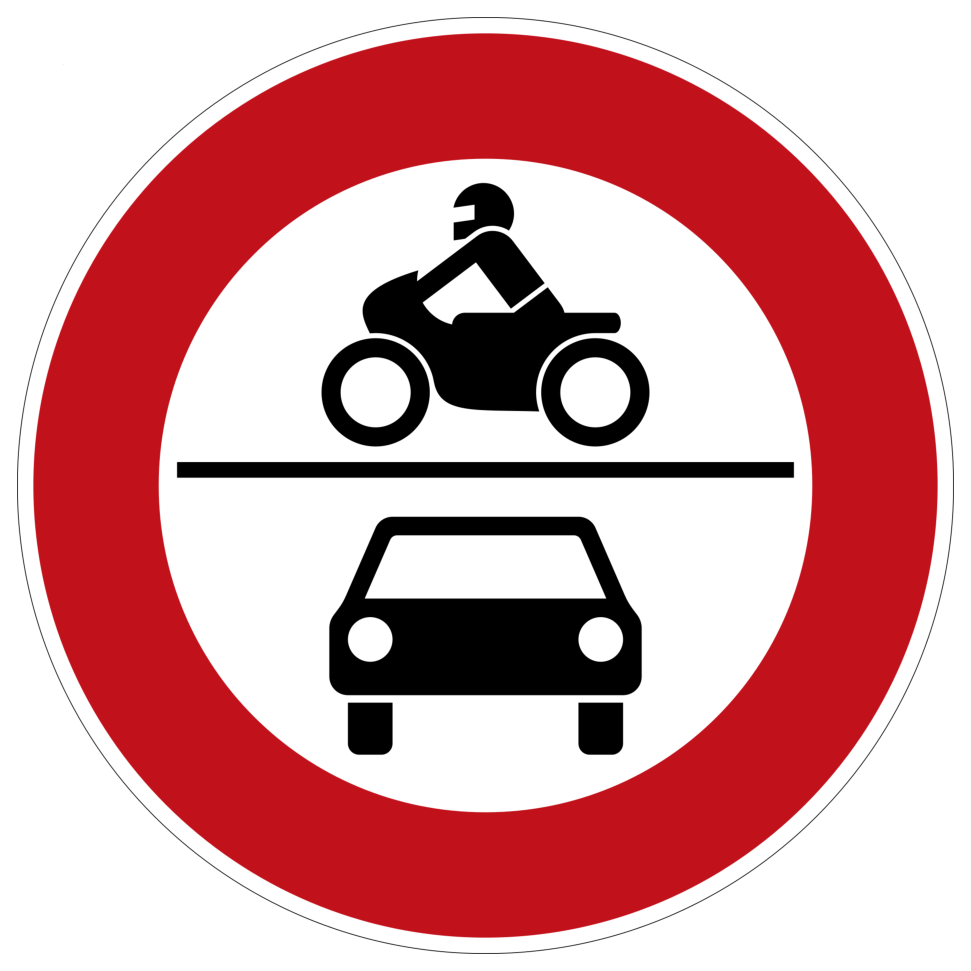
\includegraphics[scale=0.04]{{./figures/260.eps}} & Ban on motorcycles and multi-lane vehicles & 260 \\	
		
\includegraphics[scale=0.04]{{./figures/272.eps}} & No U-turn & 272 \\
		
\includegraphics[scale=0.04]{{./figures/274.eps}}& Speed limit & 274 \\
		
\includegraphics[scale=0.04]{{./figures/275.eps}}& Required speed & 275 \\
		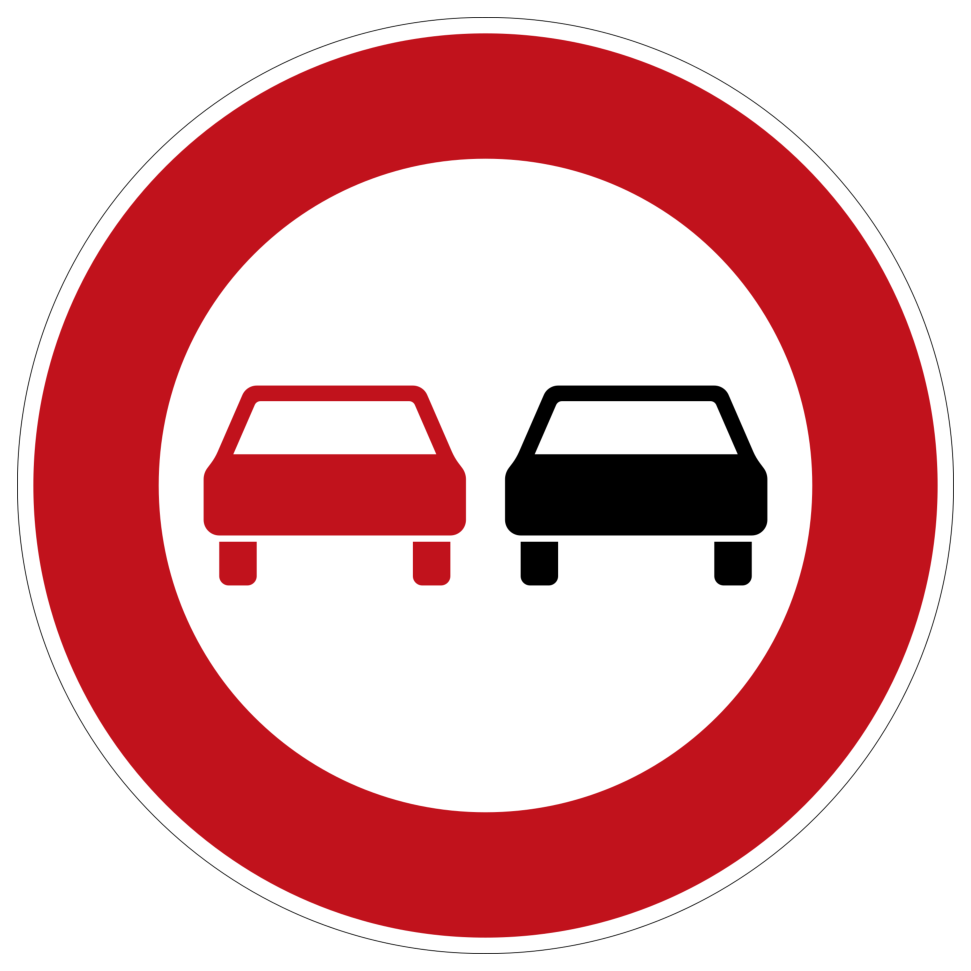
\includegraphics[scale=0.04]{{./figures/276.eps}}& No overtaking (except of non-motorized traffic participants, trains, and motorcycles without sidecar) & 276 \\
		
\includegraphics[scale=0.035]{{./figures/301.eps}} & Right of way & 301\\
		
\includegraphics[scale=0.04]{{./figures/306.eps}} & Priority road & 306\\
		
\includegraphics[scale=0.04]{{./figures/310.eps}} & Town sign & 310 \\
		
\includegraphics[scale=0.04]{{./figures/720.eps}} & Green arrow sign & 720 \\
		\bottomrule
	\end{tabular}
	\label{tab:traffic_signs}
\end{table}

\begin{table}[!htb]\centering
	\caption{Overview of all supported traffic signs. Valid for complete lanelet expresses that the traffic sign is always valid from the start of a lanelet. All traffic signs which are not mentioned in this list are valid starting starting from the end of a lanelet.}
	\ra{1.3} 
	\begin{tabular}{@{}lp{9cm}p{4cm}@{}} \toprule
		\textbf{Country} & \textbf{Traffic Sign ID} & \textbf{Valid for complete lanelet} \\ \midrule
		Germany & 101, 102, 108, 114, 123, 138, 142-10,
		201, 205, 206, 208, 209-10, \mbox{209-20}, \mbox{220-10}, \mbox{220-20}, \mbox{222-10}, \mbox{222-20} ,237, 239, 242.1, 242.2, 244.2, 
		244.2, 245, 250, 251, 253, 254, 255, \mbox{257-54}, 259, 260, 261, 262, 264, 265, 266, 26, 272, 
		274, 274.1, 274.2, 275, 276, 277, 278, 281, 282, 301, 306, 308, 310, 325.1, 
		325.2, 327, 330.1, 330.2, 331.1, 331.2, \mbox{333-21}, 333-22, 350, 357, 
		\mbox{625-10}, \mbox{625-11}, \mbox{625-12}, \mbox{625-13}, \mbox{625-20}, \mbox{625-21}, \mbox{625-22}, \mbox{625-23}, \mbox{626-10}, \mbox{626-20}, \mbox{626-30}, \mbox{626-31}, 720, 
		\mbox{1000-10}, \mbox{1000-11}, \mbox{1000-20}, \mbox{1000-21}, \mbox{1000-30}, \mbox{1000-31}, \mbox{1001-30}, \mbox{1001-31}, \mbox{1002-10}, \mbox{1002-12}, \mbox{1002-13}, 
		\mbox{1002-20}, \mbox{1002-22}, \mbox{\mbox{1002-23}, 1002-11}, \mbox{1002-14}, \mbox{1002-21}, \mbox{1002-24}, \mbox{1004-30}, \mbox{1004-31}, \mbox{1020-30}, \mbox{1022-10}, \mbox{1024-10}, \mbox{1026-36}, \mbox{1026-37}, \mbox{1026-38}, \mbox{1040-30}, \mbox{1053-33} & 
		101, 102, 108, 114, 123, 138, 142-10, 201,
		208, 209-10, 209-20, 220-10, 220-20, 222-10, 222-20, 237, 239, 242.1, 244.1, 245, 250, 251, 253, 254, 255, 257-54, 259, 260, 261, 262, 264, 265, 266, 267, 274, 274.1, 275, 276, 277,
		308, 310, 325.1, 327, 330.1, 331.1 \\
		USA & R2-1, R3-4 & R2-1 \\
		\bottomrule
	\end{tabular}
	\label{tab:supportedNationalTrafficSigns}
\end{table}


\subsection{Traffic Lights} \label{subsec:traffic_lights}
The element \textit{trafficLight} is used to represent traffic lights within the scenario (see Fig.~\ref{fig:XML_trafficLight}). Each phase/color of a \textit{trafficLight} and its duration is defined by the element \textit{cycleElement}. Similarly to the \textit{time} elements, the duration is not given as numeric value, but as integer. The color value inactive indicates that currently no phase is activated, e.g. a green right arrow traffic light can be activated iteratively. The order of the different phases is determined by the order of the \textit{cycleElements} in the element \textit{cycle}. By specifying the element \textit{timeOffset}, the cycle is shifted by this value. 

In order to define for which driving direction the traffic light is valid, i.e., the direction arrow(s) in a traffic light, the direction can be included. If the direction is not specified, the traffic light is valid for all directions. Additionally, the element \textit{active} can be used to determine whether a traffic light is active or not. Optionally, the position of the traffic sign can be included. Traffic lights are always valid starting from the end of a lanelet. 

\begin{figure}[!htpb]
	\small
	\dirtree{%
		.1 trafficLight (id).
		.2 [1] cycle.
		.3 [1..N] cycleElement.
		.4 [1] duration.
		.4 [1] color: red/redYellow/green/yellow/inactive.
		.3 [0..1] timeOffset.
		.2 [0..1] position.
		.3 [1] point.
		.2 [0..1] direction: right/straight/left/leftStraight/straightRight/leftRight/all.
		.2 [0..1] active: true/false.
	}
	\caption{Element \textit{trafficLight}.}
	\label{fig:XML_trafficLight}
\end{figure}

%The length of each state of the traffic light is specified by the elements \textit{red}, \textit{redYellow}, \textit{green} and \textit{yellow}.
\newpage
\subsection{Intersections}  \label{subsec:intersections}
The element \textit{intersection} is used to represent an intersection within the road network (see Fig.~\ref{fig:XML_intersection}). An \textit{intersection} element is defined by at least one \textit{incoming}, which consist of \textit{incomingLanelets}, \textit{outgoingsRight}, \textit{outgoingsStraight}, \textit{outgoingsLeft}, the element \textit{isLeftOf}, and the element \textit{crossing}. 

The elements \textit{outgoingsRight}/\textit{Straight}/\textit{Left} are used to infer for which lanelets the traffic light is valid for and to facilitate the calculation of priorities at intersections. The element \textit{isLeftOf} is used to infer the right-before-left-rule. The element \textit{crossing} models lanelets which cross other lanelets, e.g., crosswalks. Since all elements of a \textit{incoming} are already present in the XML file, we use an attribute referring to their unique ID. An example for an \textit{intersection} with all elements except crossings is illustrated in Fig.~\ref{fig:intersection}.
\begin{figure}[!htb]
	\centering
	\footnotesize
	\psfrag{A}[l][c]{incoming}	
	\psfrag{B}[l][c]{outgoingsRight}
	\psfrag{C}[l][c]{outgoingsStraight}
	\psfrag{D}[l][c]{outgoingsLeft}
	\psfrag{E}[l][c]{isLeftOf}
	\psfrag{F}[l][c]{crossing}
	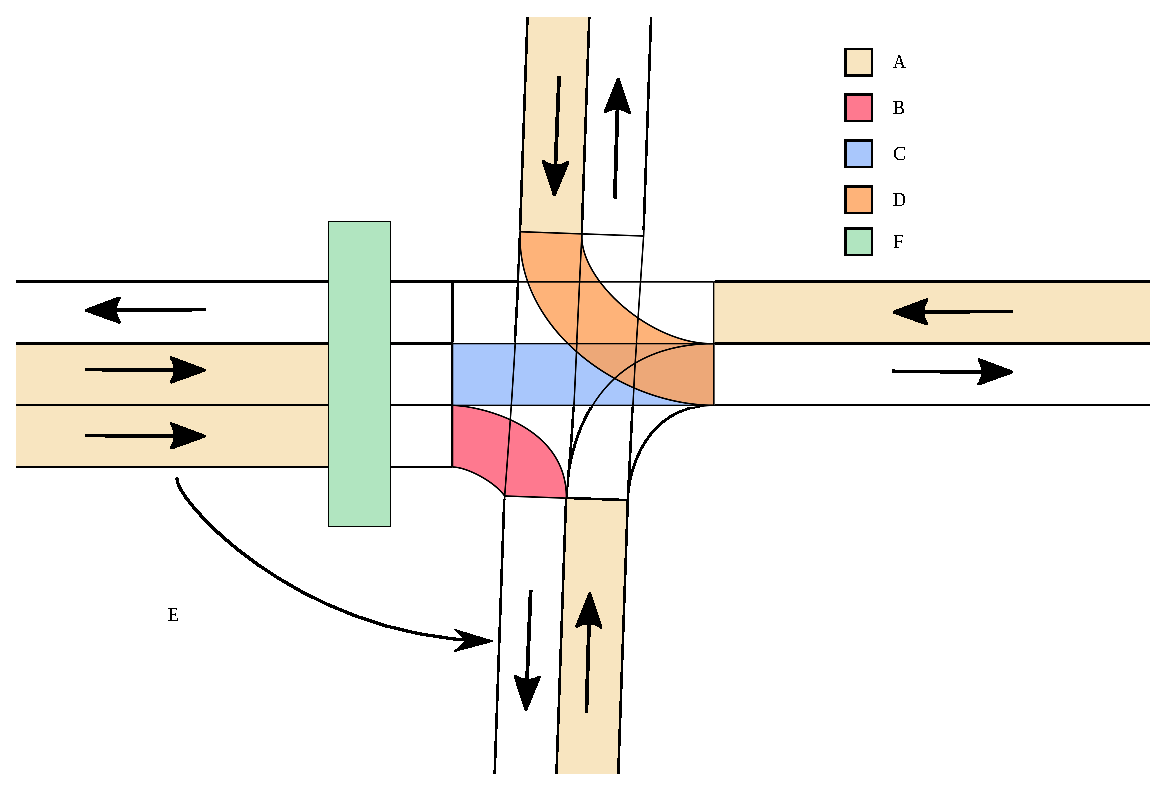
\includegraphics[width=0.6\columnwidth]{figures/intersection.eps}
	\caption{Example intersection. For better visibility, only one example lanelet is highlighted for each outgoingsRight/Straight/Left element.}
	\label{fig:intersection}
\end{figure}
\begin{figure}[!htb]
	\small
	\dirtree{%
		.1 intersection (id).
		.2 [1..N] incoming (id).
		.3 [1..N] incomingLanelet (\textrm{ref to} lanelet).
	%	.4 [0..1] stopLine.
	%	.5 [2] point.
	%	.3 [0..N] trafficSign.
	%	.3 [0..N] trafficLight.
		.3 [0..N] outgoingsRight (\textrm{ref to} all lanelets that complete the right turn within this intersection).
		.3 [0..N] outgoingsStraight (\textrm{ref to} all lanelets that are going straight).
		.3 [0..N] outgoingsLeft (\textrm{ref to} all lanelets that are turning left).
		.3 [0..1] isLeftOf (\textrm{ref to} incoming).
		.2 [0..N] crossing.
		.3 [1..N] crossingLanelet (\textrm{ref to} lanelet (usually of type crosswalk)).
	%	.3 [0..N] trafficSign.
	%	.3 [0..N] trafficLight.		
	}
	\caption{Element \textit{intersection}.}
	\label{fig:XML_intersection}
\end{figure}

\footnotetext{\href{https://commons.wikimedia.org}{commons.wikimedia.org}}

\subsection{Obstacles} \label{subsec:obstacles}
%In order to model the reality, the benchmark scenarios comprise not only lanes but different traffic participants as well. %These obstacles can be static like parked vehicles or dynamic like other vehicles driving on the road. To represent all kind of static and dynamic obstacles, different elements have been developed and are specified as follows.
The elements \textit{staticObstacle} and \textit{dynamicObstacle} are used to represent different kinds of traffic participants within the scenario. Additionally, the element \textit{environmentObstacle} is used to represent objects outside of the road network, e.g. buildings. Each obstacle element can have a \textit{type} as listed in Table~\ref{tab:obstacleTypes}.

\begin{table}[!htb]\centering
\caption{Types of obstacles.}
\ra{1.3} 
\begin{tabular}{@{}ll@{}} \toprule
\textbf{Role} & \textbf{Type} \\ \midrule
Static & parkedVehicle, constructionZone, roadBoundary, phantom, unknown \\
Dynamic & car, truck, bus, motorcycle, bicycle, pedestrian, priorityVehicle, train, phantom, unknown \\
Environment & building, pillar, median\_strip, unknown \\
\bottomrule
\end{tabular}
\label{tab:obstacleTypes}
\end{table}

The dimensions of an obstacle is specified by the element \textit{shape} (cf. Sec.~\ref{subsec:auxiliary}), and its initial configuration by the element \textit{initialState}. Additionally, the element \textit{initialSignalState} can be included, to account for properties which are not related to the dynamic of an obstacle, e.g., whether the indicators are turned on or off.

\paragraph{Initial state of obstacles}
The configuration of an obstacle at the initial time ($ t = 0$) is specified by the element \textit{initialState} with the following state variables: \textit{position}, \textit{orientation}, \textit{time}, \textit{velocity} (scalar),  \textit{acceleration} (scalar), \textit{yawRate}, and \textit{slipAngle}, as shown in Fig.~\ref{fig:XML_initialState}. 

\begin{figure}[!htpb]
	\small
	\dirtree{%
		.1 /.
		.2 initialState.
		.3 [1] position.		
		.3 [1] orientation.
		.3 [1] time.
		.4 [1] exact.
		.5 [1] $0$.
		.3 [0..1] velocity.
		.3 [0..1] acceleration.
		.3 [0..1] yawRate.
		.3 [0..1] slipAngle.
%		.3 [0..1] curvature.
%		.3 [0..1] curvatureChange.
	}
	\caption{Element \textit{initialState} of an obstacle, where each state variable (except time) can be exact or an interval.}
	\label{fig:XML_initialState}
\end{figure}

\paragraph{Initial signal state of obstacles}
The state of various signals of an obstacle at the initial time ($ t = 0$) is specified by the element \textit{initialSignalState} with the following state variables: \textit{time}, \textit{horn}, \textit{indicatorLeft}, \textit{indicatorRight},  \textit{brakingLights}, \textit{hazardWarningLights}, and \textit{flashingBlueLights}, as shown in Fig.~\ref{fig:XML_initialSignalState}. 
\begin{figure}[!htpb]
	\small
	\dirtree{%
		.1 /.
		.2 initialSignalState.
		.3 [1] time.
		.4 [1] exact.
		.5 [1] $0$.
		.3 [0..1] horn.
		.3 [0..1] indicatorLeft.
		.3 [0..1] indicatorRight.
		.3 [0..1] brakingLights.
		.3 [0..1] hazardWarningLights.
		.3 [0..1] flashingBlueLights.
	}
	\caption{Element \textit{initialSignalState} of an obstacle.}
	\label{fig:XML_initialSignalState}
\end{figure}

\subsubsection{Static Obstacles}
A static obstacle has no further information, as shown in Fig.~\ref{fig:XMLstructure}.
%\begin{lstlisting}
%<obstacle id='57'>
%	<role>static</role>
%	<type>parkedVehicle</type>
%	<shape>
%		...
%	</shape>
%</obstacle>
%\end{lstlisting}

In addition to static obstacles, traffic scenarios can contain dynamic obstacles. Please note that only elements of either of the following three behavior models may be present: with known behavior, with unknown behavior, or with unknown stochastic behavior. We do not use these different behavior models together within one traffic scenario, as indicated in Fig.~\ref{fig:XMLstructure}.

\subsubsection{Dynamic Obstacles with Known Behavior}
A dynamic obstacle with known behavior contains a trajectory of states and a series of signals (cf. Fig.~\ref{fig:XMLstructure}). 
The trajectory allows us to represent the states of a dynamic traffic participant along a path for $t > 0$. The trajectory is obtained from a dataset (whose measurements can be exact or with uncertainties), from a prediction (which generates a single trajectory for each obstacle), or created hand-crafted. The signal series is obtained from a simulator or created hand-crafted.
  
%\begin{lstlisting}
%<obstacle id='58'>
%	<role>dynamic</role>
%	<type>car</type>
%	<shape> 
%		...
%	</shape>
%	<trajectory>
%		<state>
%			...
%		</state>
%		...
%	</trajectory>
%</obstacle>
%\end{lstlisting}


\paragraph{States}
The time-discrete states of a trajectory are specified by the element \textit{state} with the following state variables: \textit{position}, \textit{orientation}, and \textit{time}, \textit{velocity} (scalar),  \textit{acceleration} (scalar), \textit{yawRate}, and \textit{slipAngle}, as shown in Fig.~\ref{fig:XML_state}. 
%Note that we optionally include acceleration as a state variable for obstacles to provide additional information, e.g. for motion prediction, even though acceleration is often used as input for vehicle models.

%\begin{lstlisting}
%<state>
%	<position>
%		...
%	</position>	
%	<orientation>
%		<exact>0.04</exact>
%		<!-- or -->	
%		<intervalStart>0.0</intervalStart>
%		<intervalEnd>0.08</intervalEnd>
%	</orientation>
%	<time>
%		<exact>0.0</exact>
%		<!-- or -->	
%		<intervalStart>0.0</intervalStart>
%		<intervalEnd>1.0</intervalEnd>
%	</time>
%	<!-- optional -->
%	<velocity>
%		<exact>15.5</exact>
%		<!-- or -->	
%		<intervalStart>15.0</intervalStart>
%		<intervalEnd>16.0</intervalEnd>
%	</velocity>
%	<!-- optional -->
%	<acceleration>
%		<exact>0.0</exact>
%		<!-- or -->	
%		<intervalStart>0.0</intervalStart>
%		<intervalEnd>-0.2</intervalEnd>
%	</acceleration>
%</state>
%\end{lstlisting} 


\begin{figure}[!htpb]
	\small
	\dirtree{%
		.1 /.
		.2 state.
		.3 [1] time.
		.3 [1] position.
		.3 [1] orientation.
		.3 [0..1] velocity.
		.3 [0..1] acceleration.
		.3 [0..1] yawRate.
		.3 [0..1] slipAngle.
%		.3 [0..1] curvature.
%		.3 [0..1] curvatureChange.
%		.3 [0..1] signalStates.
%		.4 [0..1] horn.
%		.4 [0..1] indicatorLeft.
%		.4 [0..1] indicatorRight.
%		.4 [0..1] brakingLights.
%		.4 [0..1] hazardWarningLights.
%		.4 [0..1] flashingBlueLights.
	}
	\caption{Element \textit{state} of a trajectory, where each state variable can be exact or an interval.}
	\label{fig:XML_state}
\end{figure}

\paragraph{Signal States}
The time-discrete states of a signal series are specified by the element \textit{signalState} with the following state variables: \textit{time}, \textit{horn}, \textit{indicatorLeft}, \textit{indicatorRight},  \textit{brakingLights}, \textit{hazardWarningLights}, and \textit{flashingBlueLights}, as shown in Fig.~\ref{fig:XML_signalState}.

\begin{figure}[!htpb]
	\small
	\dirtree{%
		.1 /.
		.2 signalState.
		.3 [1] time.
		.3 [0..1] horn.
		.3 [0..1] indicatorLeft.
		.3 [0..1] indicatorRight.
		.3 [0..1] brakingLights.
		.3 [0..1] hazardWarningLights.
		.3 [0..1] flashingBlueLights.
	}
	\caption{Element \textit{signalState} of a signal series.}
	\label{fig:XML_signalState}
\end{figure}


%The shape of the obstacle is not included in the trajectory, since the shape is usually not varying over time. However, time varying shapes could be included with a new element \textit{timeVaryingShape} instead of the standard \textit{shape} element, but we advise to use dynamic obstacles with unknown behavior (i.e. with occupancy elements) instead.
%\begin{lstlisting}
%<timeVaryingShape>
%	<shapeWithTime>
%		<shape>
%			...
%		</shape>
%		<time>
%			...
%		</time>
%	</shapeWithTime>
%	...
%</timeVaryingShape>
%\end{lstlisting}

\subsubsection{Dynamic Obstacles with Unknown Behavior}
For motion planning, we often do not know the exact future behavior of dynamic obstacles, but we instead represent their future behavior by bounded sets. Thus, dynamic obstacles with a unknown behavior are specified by an \textit{occupancy set}, which represents the occupied area over time by bounded sets. As shown in Fig.~\ref{fig:XMLstructure}, an \textit{occupancy set} contains a list of \textit{occupancy} elements. %, which start at $t > 0$ or $t \in [0, t^*]$, $t^* > 0$.
%\begin{lstlisting}
%<obstacle id='59'>
%	<role>dynamic</role>
%	<type>car</type>
%	<occupancySet>
%		<occupancy>
%			<shape>
%				...
%			</shape>
%			<time>
%				...
%			</time>
%		</occupancy>
%		...
%	</occupancySet>
%</obstacle>
%\end{lstlisting}

\paragraph{Occupancies}
The \textit{occupancy} element consists of a shape (occupied area) and a time, as shown in Fig.~\ref{fig:XML_occupancy}.

%\begin{lstlisting}
%<occupancy>
%	<shape>
%		...
%	</shape>
%	<time>
%		...
%	</time>
%</occupancy>
%\end{lstlisting}

\begin{figure}[!htpb]
	\small
	\dirtree{%
		.1 /.
		.2 occupancy.
		.3 [1] shape.
		.3 [1] time.
		.4 [1] exact\\OR.
		.4 [1] intervalStart.
		.4 [1] intervalEnd.		
	}
	\caption{Element \textit{occupancy} of an occupancy set.}
	\label{fig:XML_occupancy}
\end{figure}


\subsubsection{Dynamic Obstacles with Unknown Stochastic Behavior}
One can describe unknown stochastic behavior by probability distributions of states. Since many different probability distributions are used, we only provide a placeholder for probability distributions. \todo{Note that this element needs further refinement.}
\todo{Further details will follow.} 

%\begin{lstlisting}
%<obstacle id='60'>
%	<role>dynamic</role>
%	<type>car</type>
%	<shape>
%		...
%	</shape>
%	<probabilityDistribution>
%		...
%	</probabilityDistribution>
%</obstacle>
%\end{lstlisting}

%\paragraph{Probability Distribution}
%We can either describe the occupancy by bounded regions that evolve over time or by probability distributions. We approximate the probability distribution by their level sets, where each level set is modeled by a shape (e.g. polygon) and assigned with a probability.

%\begin{lstlisting}
%<probabilityDistribution>
%	...
%</probabilityDistribution>
%\end{lstlisting}

%If we describe the occupancy as a bounded set, we use a single level set with probability 1 obtained from set-based prediction\cite{Althoff2016d}.
%\begin{lstlisting}
%<occupancy>
%	<levelSet>
%		<shape>
%			...
%		</shape>
%		<probability>1</probability>
%	</levelSet>
%	<time>
%		...
%	</time>
%</occupancy>
%\end{lstlisting}

%\paragraph{Optional Tags for Obstacles}
%Elements of type \textit{tag} can be optionally added to an obstacle element, e.g. properties which might be required for some computations. They are given as a key-value pair.
%\begin{lstlisting}
%    <tag k='' v=''/>
%\end{lstlisting}
\subsubsection{Phantom Obstalces}
The element \textit{phantomObstacle} is used to specify potential occluded obstacles. Therefore, they have no trajectory, but an occupancy set.
 
 
\subsubsection{Environment Obstalces}
The element \textit{environmentObstacle} is used to specify the outline of environmental or infrastructure objects to properly compute occlusions. A \textit{environmentObstacle} is specified by its type, e.g. building, and its shape. 

\subsection{Planning Problem} \label{subsec:egoVehicles}
%The aim of the \textit{CommonRoad} benchmarks is to compare trajectory planners. Thus, 
The element \textit{planningProblem} is used to specify the initial state and one or more goal state(s) for the motion planning problem.
Note that the shape of the ego vehicle is not included in the XML scenario description, since this property depends on which vehicle parameter set is chosen (see the \textit{vehicle model documentation} on our website).
%\begin{lstlisting}
%<planningProblem id='100'>
%	<initialState>
%		...
%	</initialState>
%	<goalRegion>
%		<state>
%			...
%		</state>
%		...
%	</goalRegion>
%</planningProblem>
%\end{lstlisting}


\paragraph{Initial States}
We use the element \textit{initial state} to describe the initial state of the planning problem. In contrast to the general element \textit{state}, all state variables are mandatory and must be given exact, as shown in Fig.~\ref{fig:XML_initialState_planningProblem}. 
The element \textit{initial state} of each planning problem allows the initialization of each vehicle model, as described in more detail in our \textit{vehicle model documentation}.

%\begin{lstlisting}
%<initialState>
%	<position>
%		...
%	</position>	
%	<velocity>
%		...
%	</velocity>
%	<orientation>
%		...
%	</orientation>
%	<yawRate>
%		...
%	</yawRate>
%	<slipAngle>
%		...
%	</slipAngle>
%	<time>
%		...
%	</time>
%</initialState>
%\end{lstlisting}

\begin{figure}[!htpb]
	\small
	\dirtree{%
		.1 /.
		.2 initialState.
		.3 [1] position.
		.4 [1] point.
		.3 [1] velocity.
		.4 [1] exact.		
		.3 [1] orientation.
		.4 [1] exact.
		.3 [1] yawRate.
		.4 [1] exact.
		.3 [1] slipAngle.
		.4 [1] exact.
		.3 [1] time.
		.4 [1] exact.
		.5 [1] $0{.}0$.
		.3 [0..1] acceleration.
		.4 [1] exact.
}
	\caption{Element \textit{initial state} of a planning problem}
	\label{fig:XML_initialState_planningProblem}
\end{figure}


\paragraph{Goal States}
A planning problem may contain several elements \textit{goal state} (cf. Fig.~\ref{fig:XMLstructure}). In contrast to the general element \textit{state}, all state variables except time are optional and all variables can only be given as an interval, as specified in Fig.~\ref{fig:XML_goalState}.

\begin{figure}[!htpb]
	\small
	\dirtree{%
		.1 /.
		.2 goalState.
		.3 [1] time.
		.4 [1] intervalStart.
		.4 [1] intervalEnd.
		.3 [0..1] position.
		.4 [1..N] rectangle/circle/polygon\\OR.
		.4 [1..N] lanelet (\textrm{ref to} lanelet).
		.3 [0..1] orientation.
		.4 [1] intervalStart.
		.4 [1] intervalEnd.
		.3 [0..1] velocity.
		.4 [1] intervalStart.
		.4 [1] intervalEnd.
	}
	\caption{Element \textit{goal state} of a planning problem}
	\label{fig:XML_goalState}
\end{figure}


\section{Conclusions}

The \textit{CommonRoad} XML format is a platform-independent format for specifying road traffic scenarios for motion planning. Complex traffic situations can be encoded by specifying the road network, static and dynamic obstacles, and the planning problem. Details on models for the ego vehicle dynamics can be found in the \textit{vehicle model documentation}. Examples of traffic situations that are specified by this format can be found on the \textit{CommonRoad} website\footnote{\href{https://commonroad.in.tum.de}{commonroad.in.tum.de}}. Please contact us if you have any comments.


